\sectionnn{Introduction}

Dans le logiciel R, on peut simuler très simplement à peu près toutes les lois classiques. Dans ce TP, on se propose, pour chaque loi usuelle, de simuler des échantillons, et de calculer la moyenne et la variance de ces échantillons, ainsi que faire des graphiques représentant ces lois. Il y a quatre commandes à connaître pour chaque loi : \textbf{rmaloi} : permet de simuler selon loi, \textbf{dmaloi} : permet de calculer la densité de maloi, \textbf{pmaloi} : permet de calculer la fonction de répartition de maloi, \textbf{qmaloi} : permet de calculer le quantile de maloi.


\subsection{Exemple pour la loi normale}

  \textbf{Voir code annexe \ref{lst:normal_distribution}} : \hyperlink{\ref{lst:normal_distribution}}{Code exemple : La loi normale}

    \begin{figure}[h!]
        \centering
        \begin{subfigure}[b]{0.28\textwidth}
            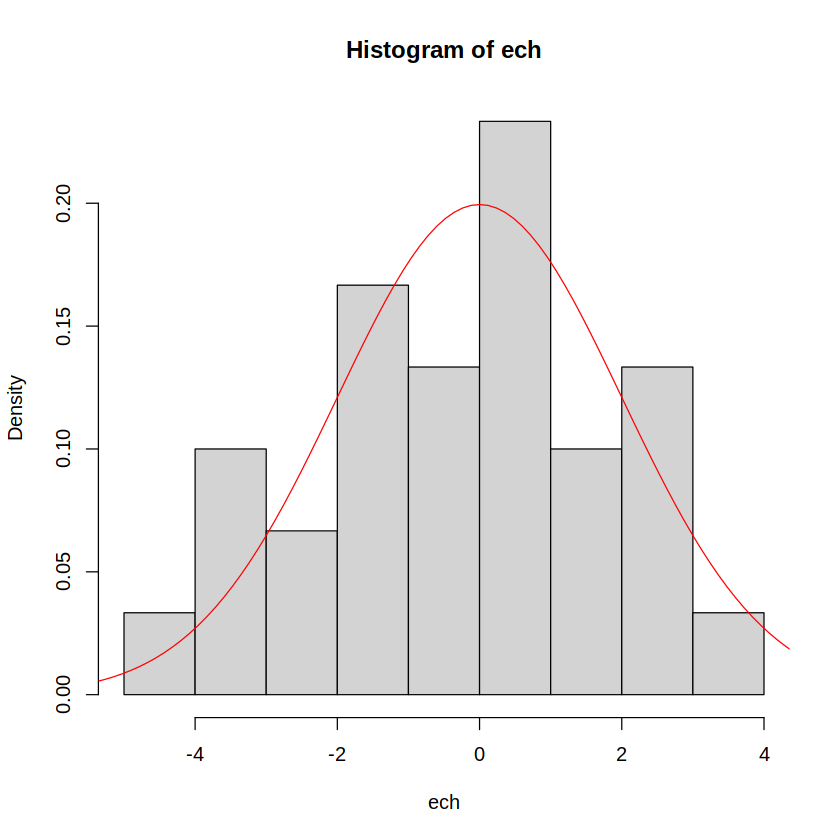
\includegraphics[width=\textwidth]{4_attachments/figures/output1.png}
            \caption{Histogramme de ech avec courbe de densité}
        \end{subfigure}
        \begin{subfigure}[b]{0.28\textwidth}
            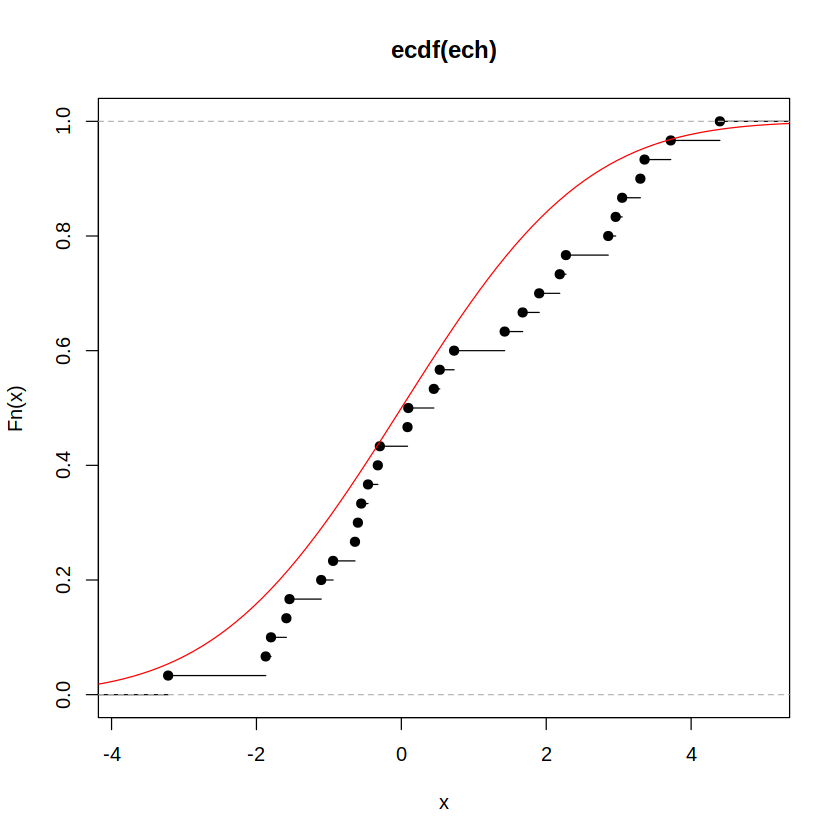
\includegraphics[width=\textwidth]{4_attachments/figures/output2.png}
            \caption{Graphique de la fonction de répartition}
        \end{subfigure}
        \caption{Graphiques pour la loi normale}
        \label{fig:normal_distribution}
    \end{figure}

    \begin{table}[H]
        \centering
        \csvautotabular{4_attachments/table/table1.csv}
        \caption{Tableau de comparaison des quantiles de la loi normale}
        \label{tab:quantile_comparison}
    \end{table}

    \subsection{Analyse des résultats}
        Dans cet exemple (voir code \ref{lst:normal_distribution}), nous avons simulé un échantillon de taille 30 selon une loi normale d'espérance $0$ et d'écart-type $2$.

        L'histogramme (Figure~\ref{fig:normal_distribution}a) montre une divergence entre la densité théorique et la simulation, due à la petite taille de l'échantillon. Cette variabilité est également visible sur le graphique de la fonction de répartition (Figure~\ref{fig:normal_distribution}b) et dans le tableau de comparaison des quantiles (Table~\ref{tab:quantile_comparison}).

        En conclusion, un échantillon plus grand est nécessaire pour une meilleure concordance avec la loi normale, conformément à la \textbf{loi des grands nombres} \cite{lawoflargeNumbers}.
\smallskip